\documentclass{article}


% This is now the recommended way for checking for PDFLaTeX:
\usepackage{ifpdf}

% Use utf-8 encoding for foreign characters
\usepackage[utf8]{inputenc}

% Swedish grammar
\usepackage[swedish]{babel}

% Setup for fullpage use
%\usepackage{fullpage}

\usepackage[a4paper]{geometry}

\usepackage[toc]{appendix}

% Space between paragraphs instead of indentation.
\usepackage{parskip}

\ifpdf
\usepackage[pdftex]{graphicx}
\else
\usepackage{graphicx}
\fi

\ifpdf
\DeclareGraphicsExtensions{.pdf, .jpg, .tif, .png}
\else
\DeclareGraphicsExtensions{.eps, .jpg}
\fi

\usepackage{float}

\pdfpxdimen=1in
\divide\pdfpxdimen by 300

%\footskip=1in
%\voffset=1in

\title{
  Projekt iMalloc \\
  Imperativ och objektorienterad programmeringsmetodik, 1DL221
}
\author{
  Niclas Edenvin \\
  Åke Lagercrantz \\
  Andreas Lelli \\
  Daniel Lindgren \\
  Elias Lundeqvist \\
  Jakob Sennerby
}

\date{2012-11-09}



\begin{document}

\maketitle

\vspace{4cm}

\begin{abstract}
  \centering
  \begin{minipage}{0.75\textwidth}
  { 
  \parskip5pt

  \noindent Det här är en rapport om en uppgift i programmeringsspråket c, i att konstruera ett eget bibliotek för minneshantering.

  \noindent Genom att dela upp uppgiften i mindre block och följa projektspecifikationen skapades en minneshanterarere med flera alternativ för hur en användare vill behandla minnet.

  \noindent Problemet löstes enligt specifikationerna och resultatet blev som väntat en effektiv minnesallokerare som används av program som vill kunna bestämma själv på vilket sätt minnet ska användas.
  }

  \end{minipage}


\end{abstract}


\newpage

\tableofcontents

\newpage

% *********************
% Infoga bild

% se Figur \ref{fig:stable}.

%\begin{figure}[H]
%  \includegraphics[width=165mm]{stabil.png}
%  \caption{Den slutliga versionen av kretsen i Logisim.}
%  \label{fig:stable}
%\end{figure}


% *************************************************************************
% *************************************************************************
% *************************************************************************
% *************************************************************************
\section{Dagbok}

\subsection{Fredag 19 Oktober}

Vi träffades hemma hos Niclas för att gemensamt gå igenom instruktionerna och förbereda oss för första projektveckan. Vi bestämde även att vi skulle använda oss av olika applikationer, tjänster och versionshanteringssystem som gör det enklare för oss att arbeta tillsammans samt hålla koll på hur vårt arbetsflöde fungerar. Vi valde att använda oss av

\begin{description} \parskip0pt
  \item[Git och github] versionshanteringssystem (ett privat repository)
  \item[Trello] strukturering av uppgifter och vem som gör vad
  \item[Tickspot] tidsrapportering
  \item[Hipchat] kommunikation och forum
  \item[Google Drive] utkast av projektdagbok och övriga dokument
  \item[\LaTeX] rapportskrivning
\end{description}
Vi började även skissa på en övergripande design för systemet för att hitta en lämplig uppdelning.

\subsection{Måndag 22 Oktober}

Vi gjorde klart den övergripande designen, se Figur \ref{fig:design}. Sedan bestämde vi oss för en gemensam kodstandard baserad på GNU coding standards\footnote{http://www.gnu.org/prep/standards/standards.html} enligt följande:

\begin{description} \parskip0pt
  \item[Tab size] 2 med soft tabs
  \item[Exempel funktionsnamn] king\_in\_danger
  \item[Exempel variabelnamn] king\_color
\end{description}

Vi delade slumpvis in oss i par och tilldelade paren varsin del av programmet och började sedan jobba i paren med headerfilerna.

\paragraph*{Andreas och Daniel} Den större delen av dagen gick åt till att planera hur projektet skulle vara utformat. Vi började arbeta på skräpsamlingen och test för dessa.

\paragraph*{Elias och Jakob} Gick igenom hur minneshanteringen kommer fungera på representationsnivå. Diskuterade en del med Åke och Niclas också och kommer inte fram till någon vettig lösning. Vi pratade med våran coach Niklas också och han sa att han inte har fått tillräckligt med info för att hjälpa oss med detta. Vi mailar Tobias för att se vad han har att säga.

\paragraph*{Niclas och Åke} Gjorde makefile och skelett till unittesting. Försökte lösa designproblemet med hur refcount och de privata managed- och manualobjekten ska hanteras.


\begin{figure}[H]
  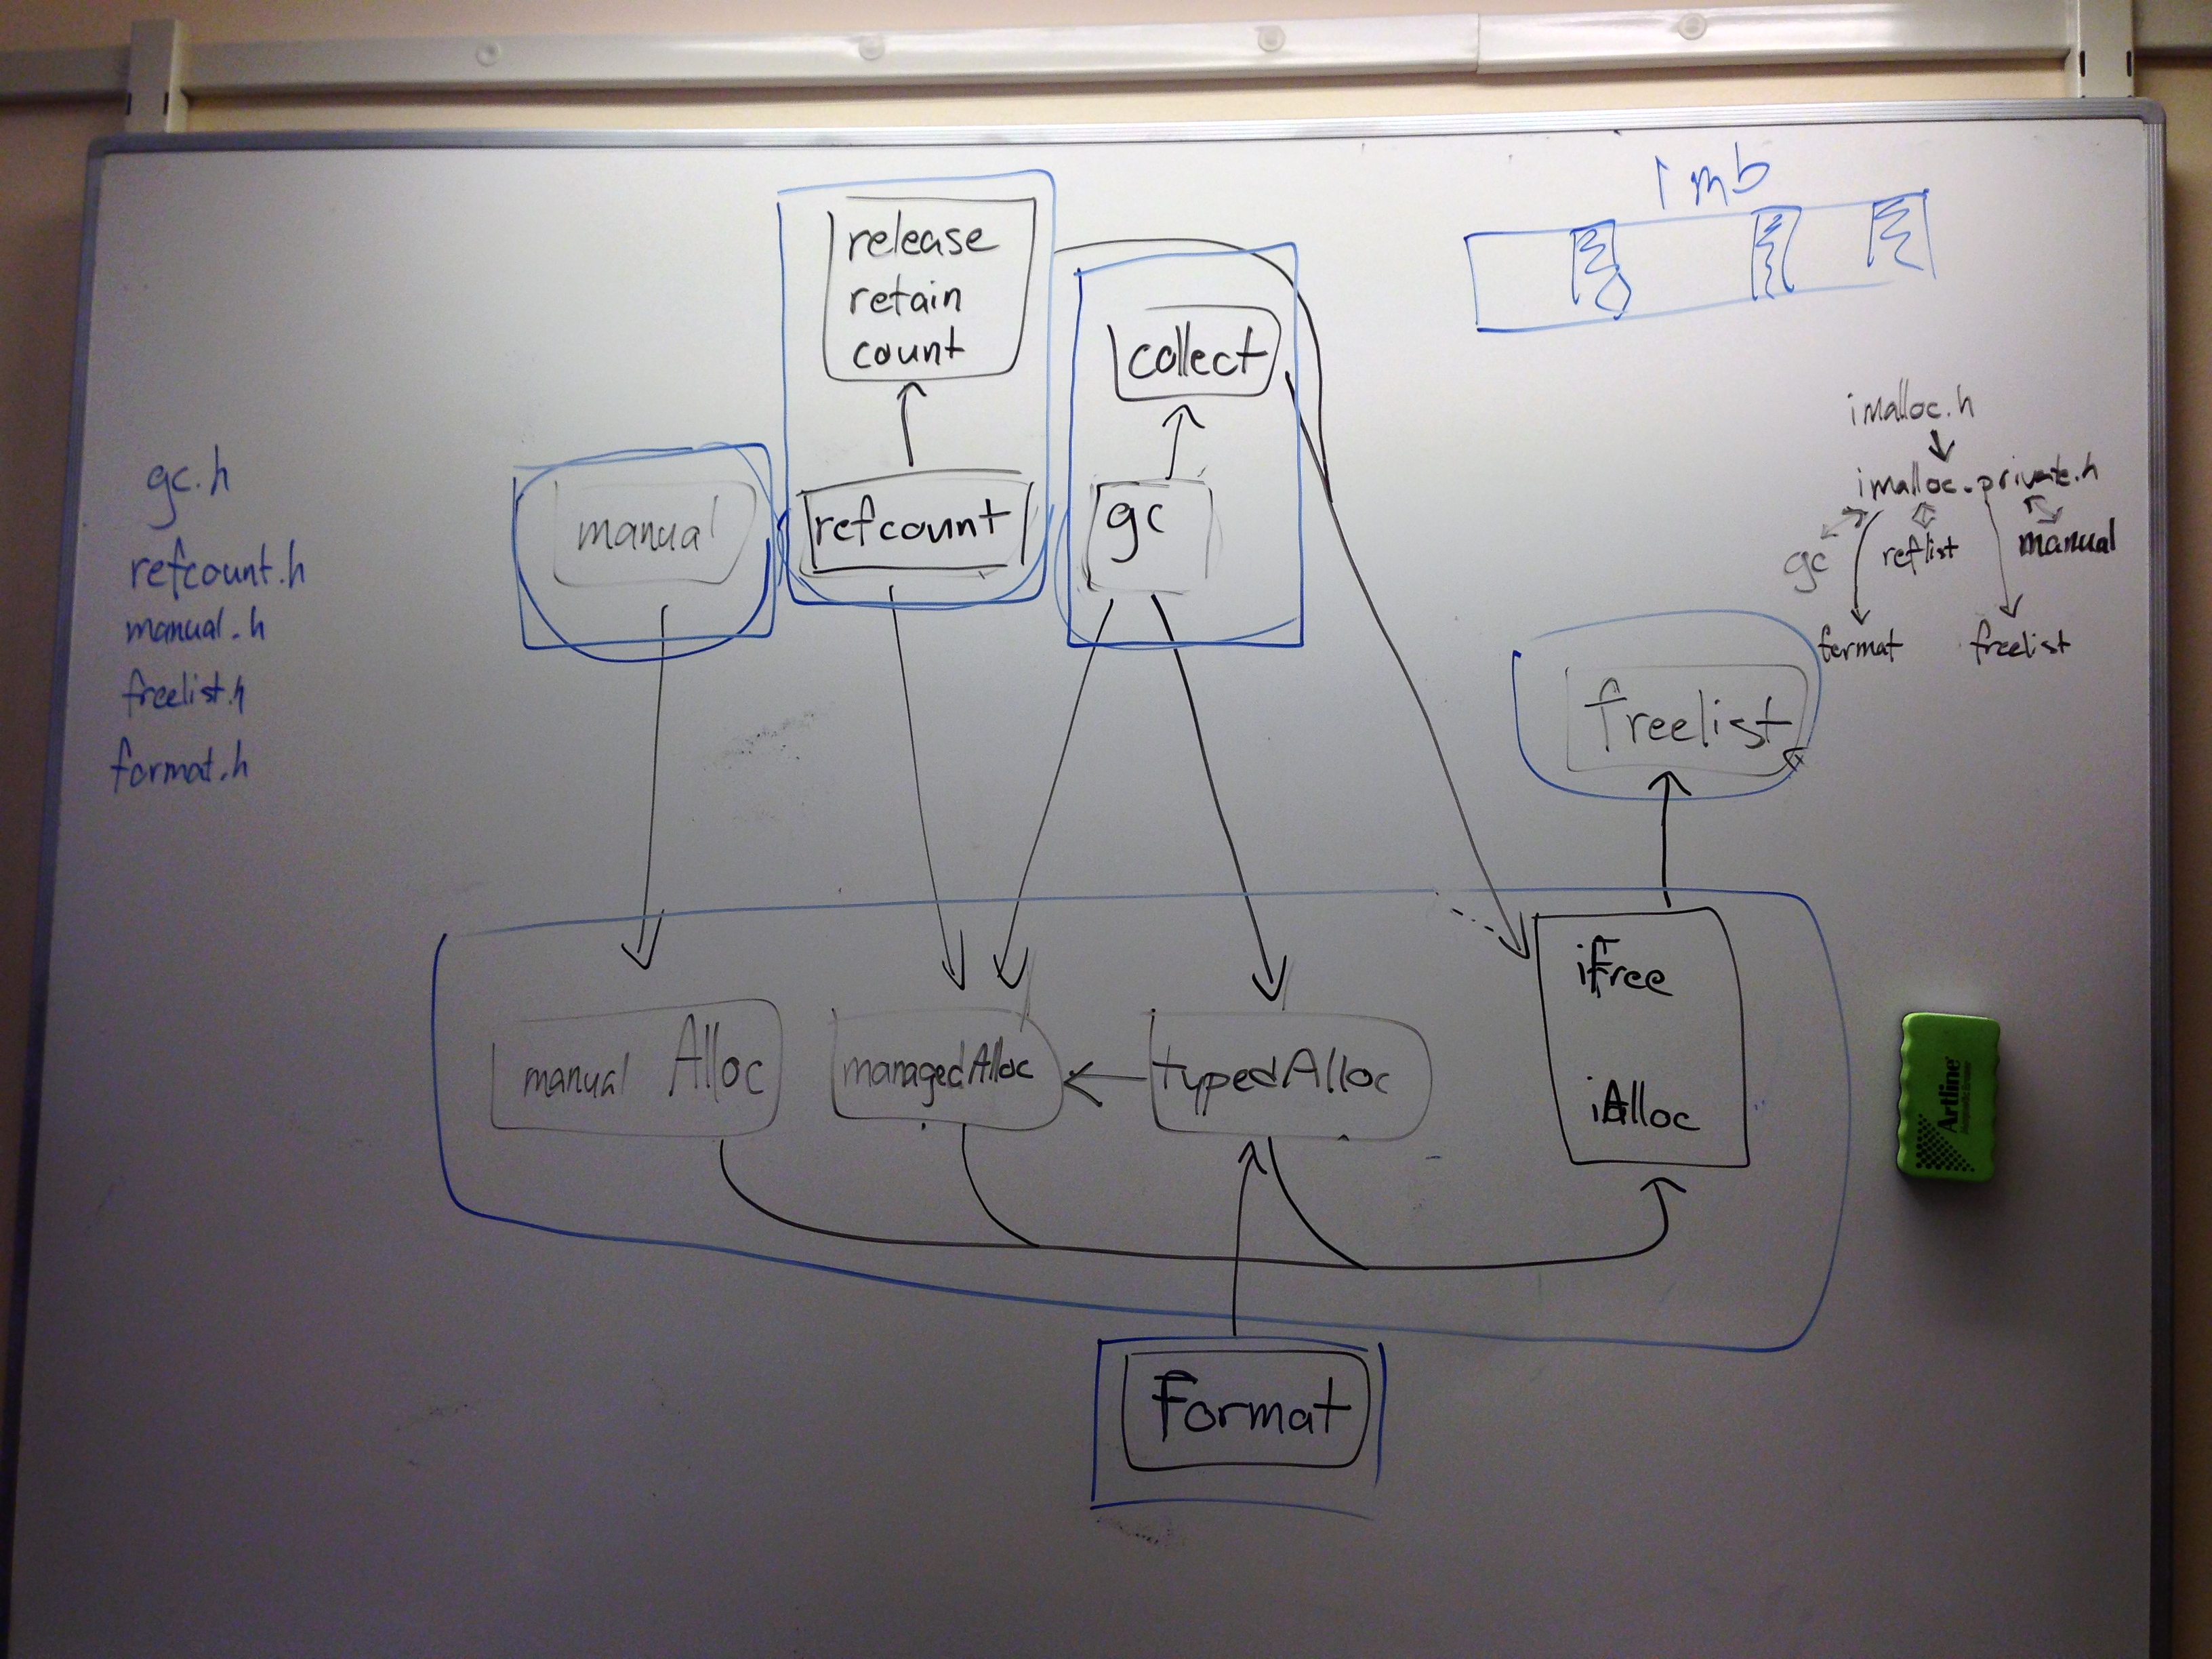
\includegraphics[width=\columnwidth]{images/design_whiteboard.jpg}
  \caption{Den ursprungliga designen och indelningen.}
  \label{fig:design}
\end{figure}

\subsection{Tisdag 23 Oktober}

\paragraph*{Andreas och Daniel} Vi fortsatte arbeta på gc och diskuterat på vilket sätt den borde fungera. Koden för att traversera stacken har inte delats ut ännu, av denna anledning är det svårt att få våra testfall att fungera som de bör (Då vi ej kan traversera stacken på ett vettigt sätt utan att se vilka pekare som leder dit).

\paragraph*{Elias och Jakob} Vi satt fast och kunde inte riktigt koda någonting på grund av att vi inte visste hur vi skulle representera våran freelist, alloclist och refcount. Vi väntade på svar från Tobias men började koda på formatstring så länge.

Vi blev klara med formatstring och alla tester till denna innan samtliga i gruppen gick och pratade med Justin Pearsson. Justin berättade att vi skulle “gömma” freelist och alloclist innan stylen och även refcount skulle “gömmas” innan objektet. Vi började arbeta med refcount igen och gjorde klart det mesta förutom release-delen. Vi kunde inte riktigt arbeta mer då vi behöver färdig kod för “ifree”. Därför har nu release och testkoden en del placeholders.

\paragraph*{Niclas och Åke} Fortsatte på funktioner i memory. Fixade unittests så att alla kan skriva tester. Tillämpade TDD och par-switching (highfive!). Vi gick även och pratade med Justin som tyckte att det var helt ok att göra som vi tänkt att spara refcount direkt innan varje objekt på heapen, trots att programmeraren då förlorar en del minne.


\subsection{Onsdag 24 Oktober}
\paragraph*{Andreas och Daniel} Idag arbetade vi med gc.c och främst funktioner för traversering och markering av element på heapen. Vi fastnade en del på hur vi skulle göra med de element på heapen som var en pekare till andra element inom adressrymden, i början valde vi att spara allt på en lista och sedan markera dem en och en men ändrade oss sedan till att använda rekursion. Vi är snart även klara med Sweep-delen av algoritmen, dvs den delen då vi friar upp de objekt som inte har blivit markerade som använda.

\paragraph*{Jakob och Elias} Eftersom vi inte kan slutföra refcount på grund av att release inte har funktioner tillräckligt för att free:a korrekt så har vi nästan gjort färdigt priv\_imalloc idag, det saknas lite tester. Efter två timmars diskuterade om hur exemplen som finns i projektspecen var tänkt att fungera så gick vi och Åke till Wrigstad och fick konstaterat för oss att det var som vi trodde, dvs fel i specen.

\paragraph*{Niclas och Åke} Vi fortsatte på funktioner och tester av memory. Vi försökte också komma på hur vi ska göra med cross-referencing som vi har på vissa ställen.

\subsection{Torsdag 25 Oktober}

\paragraph*{Andreas och Daniel} Idag har vi arbetat en hel del på funktionerna för att traversera heapen, Swipe algoritmen och markeringsalgoritmen. Vi har fått det mesta att fungera och börjat felsöka. Vi behöver dock funktionen för att traversera Stacken innan vi kan säga att GC är helt klar men det borde inte vara mycket arbete kvar här nu!

\paragraph*{Jakob och Elias} Har jobbat med priv\_imalloc för det mesta idag. Det har gått bra. Vi är nästan färdig med implementationen av själva imalloc-funktionen. Har mest felsökning kvar. Sedan kan vi förhoppningsvis börja med priv\_free (a.k.a ifree) så vi kan slutföra refcount.


\paragraph*{Niclas och Åke} Arbetat med tester och funktioner i memory. Löst problemet med cross-referencing av headerfiler. Designändringar i vissa structs gällande memory. Implementerat en privat headerfil för memory, så att vi kan testa våra privata hjälpfunktioner med enhetstestning.

\subsection{Fredag 26 Oktober}

\paragraph*{Andreas och Daniel} Vi har först och främst gjort klart GC, vi har implementerat funktionerna för att traversera stacken och allting kompilerar som det sig borde. Vi måste dock fixa våra testfall då dessa inte längre fungerar på grund av att vi har ändrat hur minnet beter sig. Dessutom kräver testerna (för att kunna testa vettiga saker) att iMalloc är mer eller mindre klar, detta eftersom att gc ska “städa undan” data genererad av användaren. Vi har kollat på olika program för koddokumentation och de bäst lämpade tycks vara Doxygen som vi började arbeta med då det kan generera \LaTeX-kod. Vi har även hunnit göra två stycken “flow charts” för hur de olika modulerna kommunicerar med varandra.

\paragraph*{Jakob och Elias} Precis som igår arbetade vi idag med priv\_imalloc, vi skrev klart alla funktioner samt skrev tester som vi tidigare inte kunnat skriva pga. de okompletta memory-funktionerna. Nu återstår bara en del småfix och felsökning.

\paragraph*{Niclas och Åke} Implementerat memory\_claim och diverse underfunktioner. Tester för desamma. Memory känns nu mer eller mindre klart, finns en del småfix och felsökning att genomföra.

\subsection{Måndag 29 Oktober}
\paragraph*{Samtliga} Idag träffade vi vår coach Niklas för ett avstämningsmöte. Vi roterade även parkombinationerna och under den här veckan kommer följande par att arbeta:

\begin{description} \parskip0pt
  \item[Andreas och Niclas] Dokumentation
  \item[Jakob och Åke] priv\_imalloc
  \item[Daniel och Elias] garbage collection
\end{description}

Arbetsfördelningen kommer att variera en del under veckan då de flesta av våra funktioner är mer eller mindre färdiga.

\paragraph*{Andreas och Niclas} Vi började under dagen bygga upp all dokumentation som ska in. Vi har helt enkelt börjat sammanställa all tidsrapportering, alla övergripande designdokument etc och sammanställt detta till en inlämningsbar rapport.

\paragraph*{Elias och Daniel} Idag har vi jobbat med gc-delen, det blev vi som fick fortsätta med den efter rotationen. Elias fick lite tid att sätta sig in i koden och efter det släppte Jakob och Åke ut ny kod till priv\_imalloc. Detta resulterade i att vi fick modifiera vår kod då priv\_imalloc nu hade olika funktioner för managed och manual alloc, något den inte hade tidigare. Detta gjorde att vi fick en del problem att kompilera vår kod. Därefter löste Åke och Jakob lite problem, varpå vi kunde ändra tillbaka vår kod till den ursprungliga. Vi fick koden att fungera som det var tänkt men det saknas fortfarande tester, något vi inte har kunnat göra då vi behöver ha iMalloc helt färdigskriven.

\paragraph*{Jakob och Åke}
Skrev fler tester för priv\_imalloc samt spenderade mycket tid på att debugga kod här och var. Alla började bli typ klara med sina delar och vi försökte sätta ihop och testa dem tillsammans.

\subsection{Tisdag 30 Oktober}

\paragraph*{Andreas och Niclas}
Under dagen arbetade vi en del med koddokumentation men gick sedan över till att bygga upp de dokument vi skall lämna in i \LaTeX. Vi har lagt in dagboken, arbetat på diverse stapeldiagram för att visa tidsfördelningen och under processen även lärt oss hur man arbetar i \LaTeX!

\paragraph*{Daniel och Elias}
I väntan på att Åke och Jakob ska bli färdig med priv\_imalloc så har vi börjat skriva på den övergripande designdokumentationen. Vi har haft problem med att förstå vad man ska få med och hur, men vi har skrivit det så bra vi kan utifrån vår tolkning. Efter det kom vi igång med gc:s test igen och satt med det resten av dagen.

\paragraph*{Jakob och Åke}
Skrev klart sista delarna av priv\_imalloc inkl tester. Fortfarande massor av buggar. 32-bitars minnesadresser i traverse\_heap på 64-bitarsmaskiner, varifrån kommer dem?

\subsection{Onsdag 31 Oktober}
\paragraph*{Andreas och Niclas}
Under dagen arbetade vi med de dokument vi skall lämna in, vi har fortsatt formatera allt i \LaTeX, ordnat med graferna och gjort klart den övergripande designen. Vi felsökte också GC tillsammans med de andra grupperna.

\paragraph*{Daniel och Elias}
Idag har vi ägnat all tid åt felsökning av GC. Vi har problem när vårt test för GC:n har skräp att samla.

\paragraph*{Jakob och Åke}
Debuggade gc-delen. Skrev om stora delar av traverse\_heap. Olika problem på olika platformar. BUS error på SPARC, segfaults på x86.

\subsection{Torsdag 1 November}
\paragraph*{Andreas och Niclas} Vi har delvis vart med och diskuterat fel i GC men främst har vi arbetat med koddokumentation på gränssnittsnivå och övriga dokument som skall lämnas in.

\paragraph*{Daniel och Elias} Vi har även idag ägnat all tid åt felsökning i GC. Vi löser fler och fler fel men det dyker alltid upp nya. Har fått mycket hjälp från de andra grupperna då de har ungefär samma problem.

\paragraph*{Jakob och Åke} Fixat massa buggar i gc. Nu stegar vi bla. rätt längd i traverse\_heap oavsett platform.

\subsection{Fredag 2 November}
\paragraph*{Andreas och Niclas} Samma som tidigare dagar, koddokumentation på gränssnittsnivå, finslipning av de dokument vi ska lämna in.

\paragraph*{Daniel och Elias} Debuggande (som hela denna vecka). Sen övergick vi till att skriva på dokumentationen. Elias jobbade främst på reflektionen över grupparbetet medan Daniel började med ett dokument om gränssnitten mellan modulerna.

\paragraph*{Jakob och Åke} Fortsätter med debugging men kommer inte riktigt någonstans. Hittade ett sätt att skriva ut hela stacken i gdb men hjälpte inte så mycket. Nya tag på Måndag!

\subsection{Söndag 4 November}
\paragraph*{Åke} Listade ut var våra spökpekare kommer ifrån. De ligger kvar på stacken från tidigare stackframes som återanvänds utan att all data i stackframen skrivs över.

\subsection{Måndag 5 November}
\paragraph*{Andreas och Niclas} Vi har arbetat på koddokumentationen på gränssnittsnivå och mer eller mindre skrivit klart reflektionen. Tillsammans med övriga har vi varit uppe och pratat med Elias Castegren och Justin Pears beträffande de sista problemen vi haft med vår kod.

\paragraph*{Daniel och Elias} Idag har Elias fokuserat främst på att skriva dokumentation och börjar bli klar med de första utkasten nu och ska sedan börja finslipa på allt. Daniel har arbetat med buggarna i GC samt skrivit lite mer på gränsnitten mellan modulerna.

\paragraph*{Åke} Lyckades ta bort många av spökpekarna genom att innan collect anropas rensa stacken ovanför från pekare. En spökpekare återstod dock vid normal körning, men denna försvinner mystiskt när programmet stegas igenom gdb. Detta leder oss till att tro att det kan vara en pekare som ligger i ett register som inte töms. Exprimentering med jmp\_buf ledde dock ingen vart. Vi bestämde oss för att anse att problemet inte är så viktigt då pekarna i ett verkligt scenario skulle skrivas över förr eller senare och på så sätt tas bort som skräp. Det är ju bara enhetstesterna som strular på vissa platformar, inte själva koden.

\paragraph*{Jakob} Var bollplank åt Åke.

\subsection{Tisdag 6 November}
\paragraph*{Daniel} Skrev på gränsnitten mellan modulerna.

\paragraph*{Andreas} Arbetade med koddokumentation på gränssnittsnivå och reflektion. Vi pratade även med Tobias efter föreläsningen om vårt problem betr. skräp på stacken. 

\paragraph*{Jakob} Sjuk.

\paragraph*{Niclas} Arbetat på koddokumentationen på gränssnittsnivå.

\paragraph*{Åke} Skrev på reflektion \& dokumentation.

\paragraph*{Elias} Skrivit reflektion.

\subsection{Onsdag 7 November}

% *************************************************************************
% *************************************************************************
% *************************************************************************
% *************************************************************************
\section{Parrotationer}
Den första dagen jobbade alla tillsammans, gick igenom instruktionerna och diskuterade uppgiften. Innan någon form av uppdelning i par kunde göras så krävdes en tydlig struktur på uppgiften med en logisk uppdelning av arbetsuppgifter. Därför ägnades hela första dagen åt planering.

\subsection{Vecka 1}
Dag två började med uppdelning av par baserat på den övergripande designen som gjorts under första dagen. En slumpgenerator användes för att dela upp gruppen i par om två samt vilken arbetsuppgift varje par skulle ansvara för.
Parindelningen för vecka 1 såg ut så här:

\begin{description} \parskip0pt
  \item[Niclas och Åke] memory
  \item[Elias och Jakob] refcount
  \item[Andreas och Daniel] garbage collection
\end{description}

Mer detaljerade beskrivningar av koddelarna finns i bilaga \ref{appendix:design}.

\subsection{Vecka 2}
Alla räknade med att arbetsfördelningen skulle variera under andra veckan då flera av de stora delarna skulle vara klara. Rotation av parindelning skedde precis som under första veckan med hjälp av slumpgenerator. Det slumpades även om vilka som skulle sitta kvar med samma uppgift som tidigare. 
Parindelning vecka 2 såg ut så här:

\begin{description} \parskip0pt
  \item[Andreas och Niclas] dokumentation
  \item[Jakob och Åke] priv\_imalloc
  \item[Daniel och Elias] garbage collection
\end{description}

\subsection{Vecka 3}
När vecka 3 drog igång var all kodskrivning i princip klar. Därför blev vecka 3 utan bestämda par och det jobbades mer flytande.

% *************************************************************************
% *************************************************************************
% *************************************************************************
% *************************************************************************
\section{Tidsåtgång}

Under projektets gång har alla arbetat med ett program för “time tracking” som heter Tickspot. Efter varje arbetsdag rapporterade alla in hur många timmar vardera person hade arbetat samt vilken del som det jobbats på.

Totalta arbetstiden för projektet är 230, varav 6 timmar på möten, x timmar på dokumentation, x timmar på planering samt x timmar på implementation och testning.

Då alla har försökt jobba enligt TDD (Test Driven Development) har det varit svårt att räkna ut hur mycket tid som gick specifikt till testerna utan vi ser det som en del av implementationen. Nedan följer två diagram där arbets- och tidsfördelningen är tydlig.

\begin{figure}[H]
  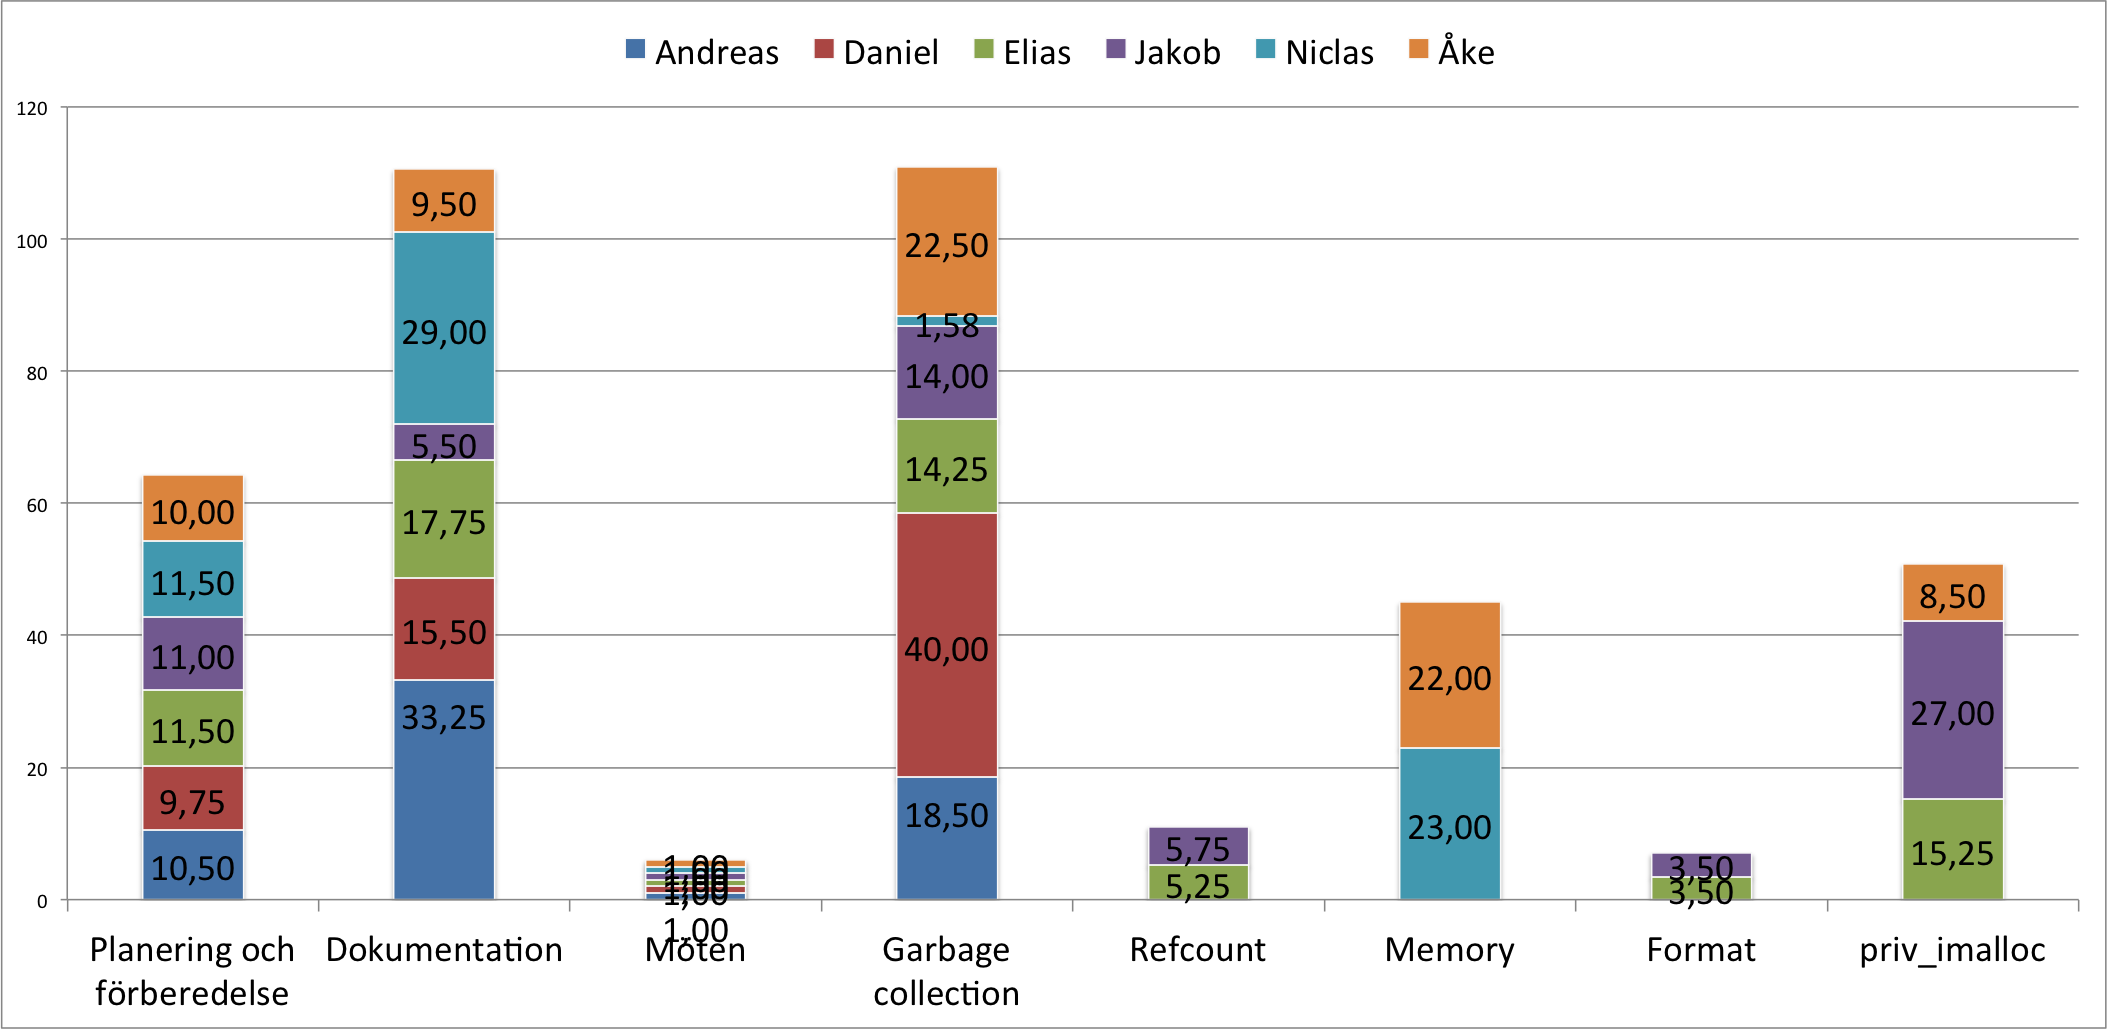
\includegraphics[width=\columnwidth]{images/chart_parts.png}
  \caption{Tidsfördelningen över projektets olika delar 
    samt vem som arbetat på vad.}
  \label{fig:chart_parts}
\end{figure}

\begin{figure}[H]
  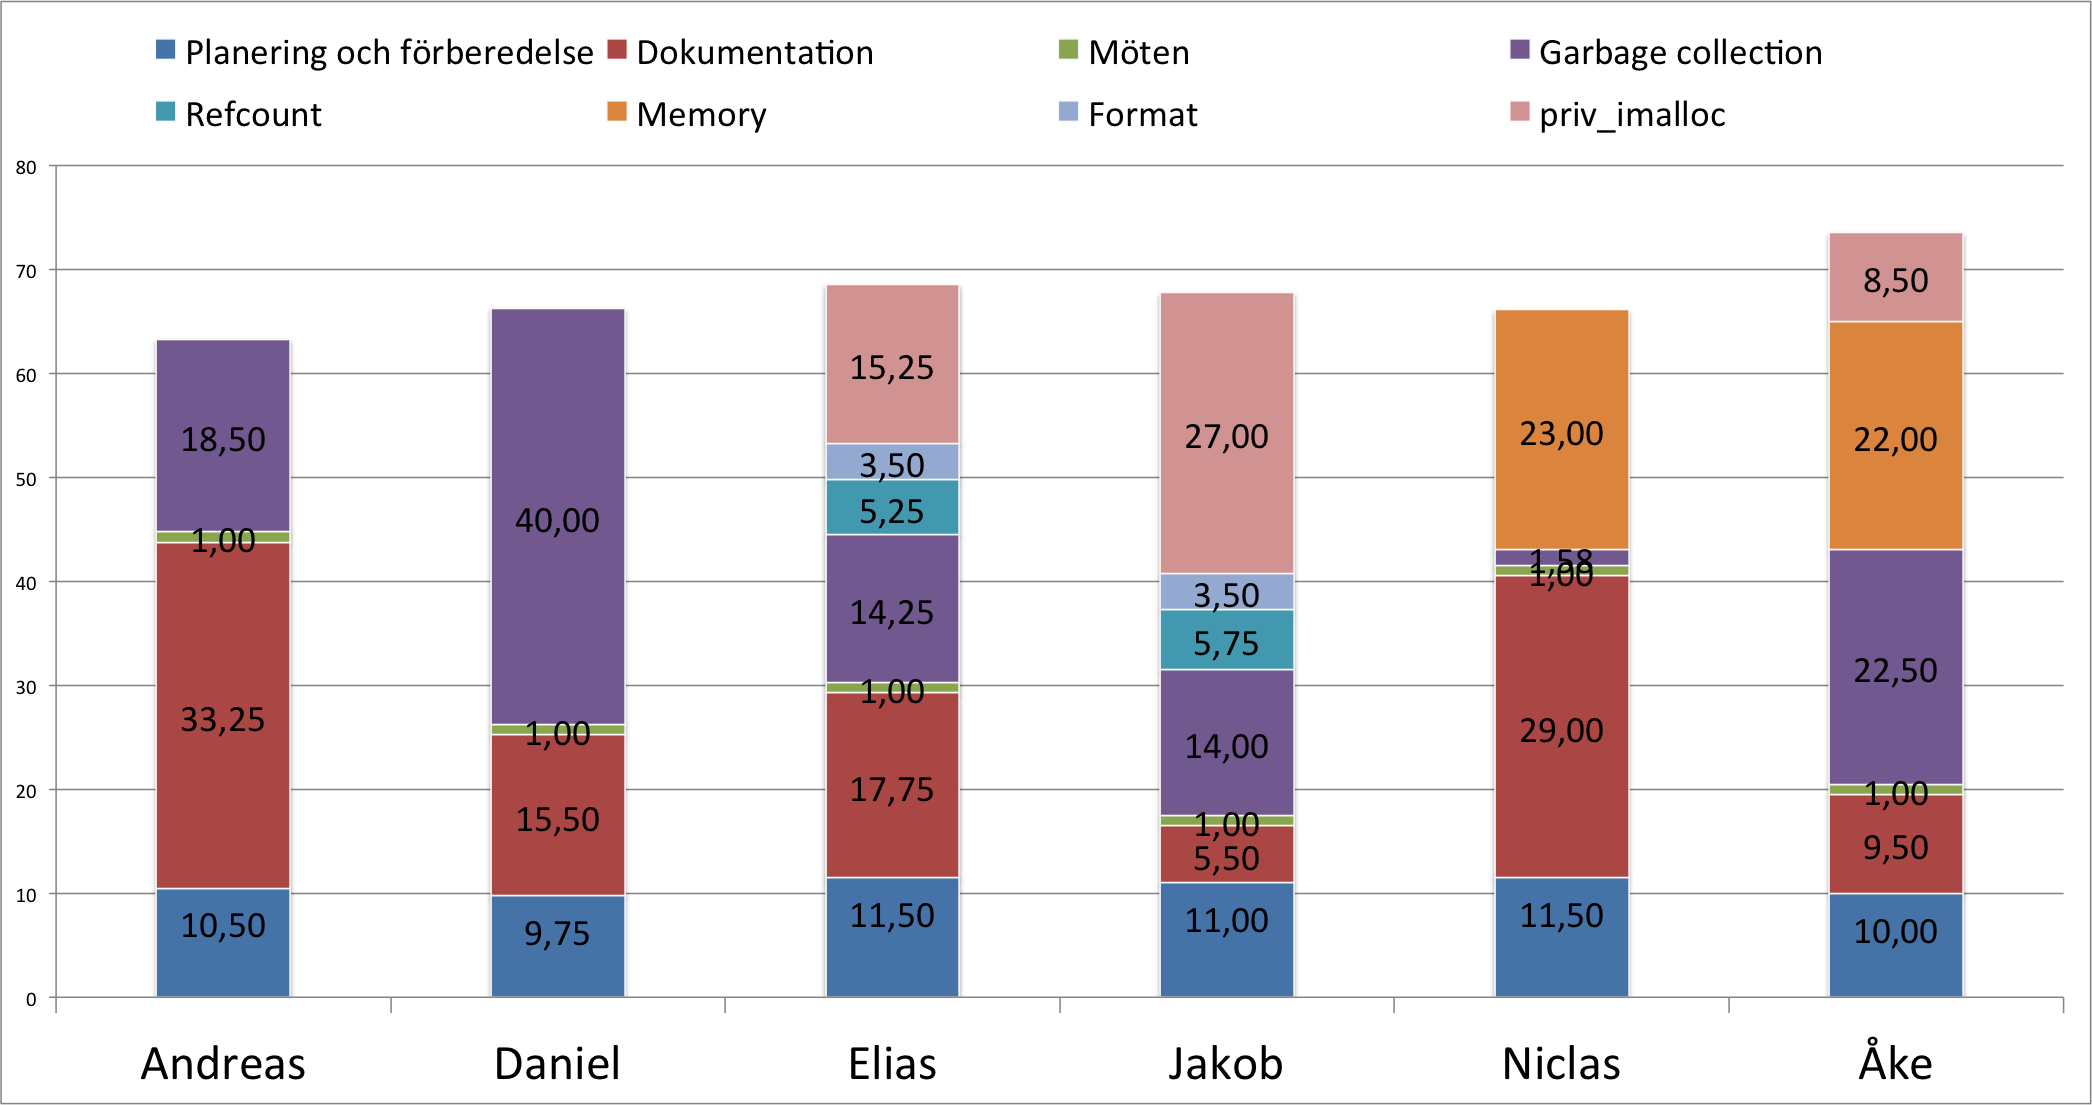
\includegraphics[width=\columnwidth]{images/chart_people.png}
  \caption{Personlig tidsfördelning över de olika delarna av projektet.}
  \label{fig:chart_people}
\end{figure}


% *************************************************************************
% *************************************************************************
% *************************************************************************
% *************************************************************************
\section{Brister}

Vår lösning är fullt fungerande förutom enhetstester som använder sig av funktionen collect(). Alla underfunktioner till allokeringen sparar temporär data på stacken, bland annat pekare till vår adressrymd på heapen. När dessa funktioner returnerar flyttas stackpointern ner och de stackframes som innehåller den temporära datan ligger utanför den allokerade delen av stacken. Problemet uppstår när traverseStack() ligger djupare i anropsledet, vilket betyder att vi återanvänder nämnda stackframes. I vissa fall kommer data i dessa stackframes inte att skrivas över, och vi har på så sätt fått skräpdata på den aktiva stacken som leder till att objekten som datan pekar till markeras som levande när de egentligen är skräp.

I ett verkligt scenario är detta inte ett problem då skräpet förr eller senare skrivs över på stacken och försvinner, men det gör det svårt att tillverka enhetstester med förutbestämt beteende. Vi testade att precis innan collect() anropas rensa stacken ovanför \$sp, vilket rensade ut nästan allt skräp.

En skräppekare återstod dock i vanlig körning, men försvann mystiskt när koden stegades igenom i debuggern. En tanke är att denna pekare ligger kvar i något register som inte nollställs.

% *************************************************************************
% *************************************************************************
% *************************************************************************
% *************************************************************************
\section{Bilagor}
\appendix
\section{Övergripande designdokument}
\label{appendix:design}


% *********************
% Infoga bild

% se Figur \ref{fig:stable}.

%\begin{figure}[H]
%  \includegraphics[width=165mm]{stabil.png}
%  \caption{Den slutliga versionen av kretsen i Logisim.}
%  \label{fig:stable}
%\end{figure}


% *************************************************************************
% *************************************************************************
% *************************************************************************
% *************************************************************************


Projektet är uppdelat i fem stora delar: priv\_imalloc, refcount, gc, memory och utilities. Det kändes som en naturlig uppdelning. Memory var från början från början kallad freelist, men ändrades sedan till att kallas för memory då den modulen hanterar allt som rör freelistan samt alloclistan (listan med allokerade objekt). Utilities skapades för att tillåta användning av boolean och för att komma åt refcounten (sparad som metadata).

De olika delarna är inte exakt lika stora och omfattande men är viktiga för att få en logisk struktur på projektet.

Vi delade upp programmet baserat på hur de olika delarna hänger ihop med varann. Vi försökte lyfta ut kod som används av flera moduler i separata block så vi slipper upprepad kod. Till exempel vill vi kunna använda chunklistorna i de flesta moduler. Vi tänkte också på att varje block skulle kunna skrivas oberoende av hur de andra såg ut, även om detta inte alltid var helt möjligt. På så sätt blev det lättare att skriva tester innan man började koda då man inte behövde tänka på hur miljön såg ut utanför ens egen modul.

I början tyckte vi att den “indelning” som stog i projektspecifikationen kändes relativt bra, dvs att dela upp minneshantering med alloc och free, referensräknaren och garbage collection i tre block, men valde sedan att dela upp det ytterligare, exempelvis lämpade sig inte delen med alloc och free att vara en egen del då den var så liten.



\begin{figure}[H]
  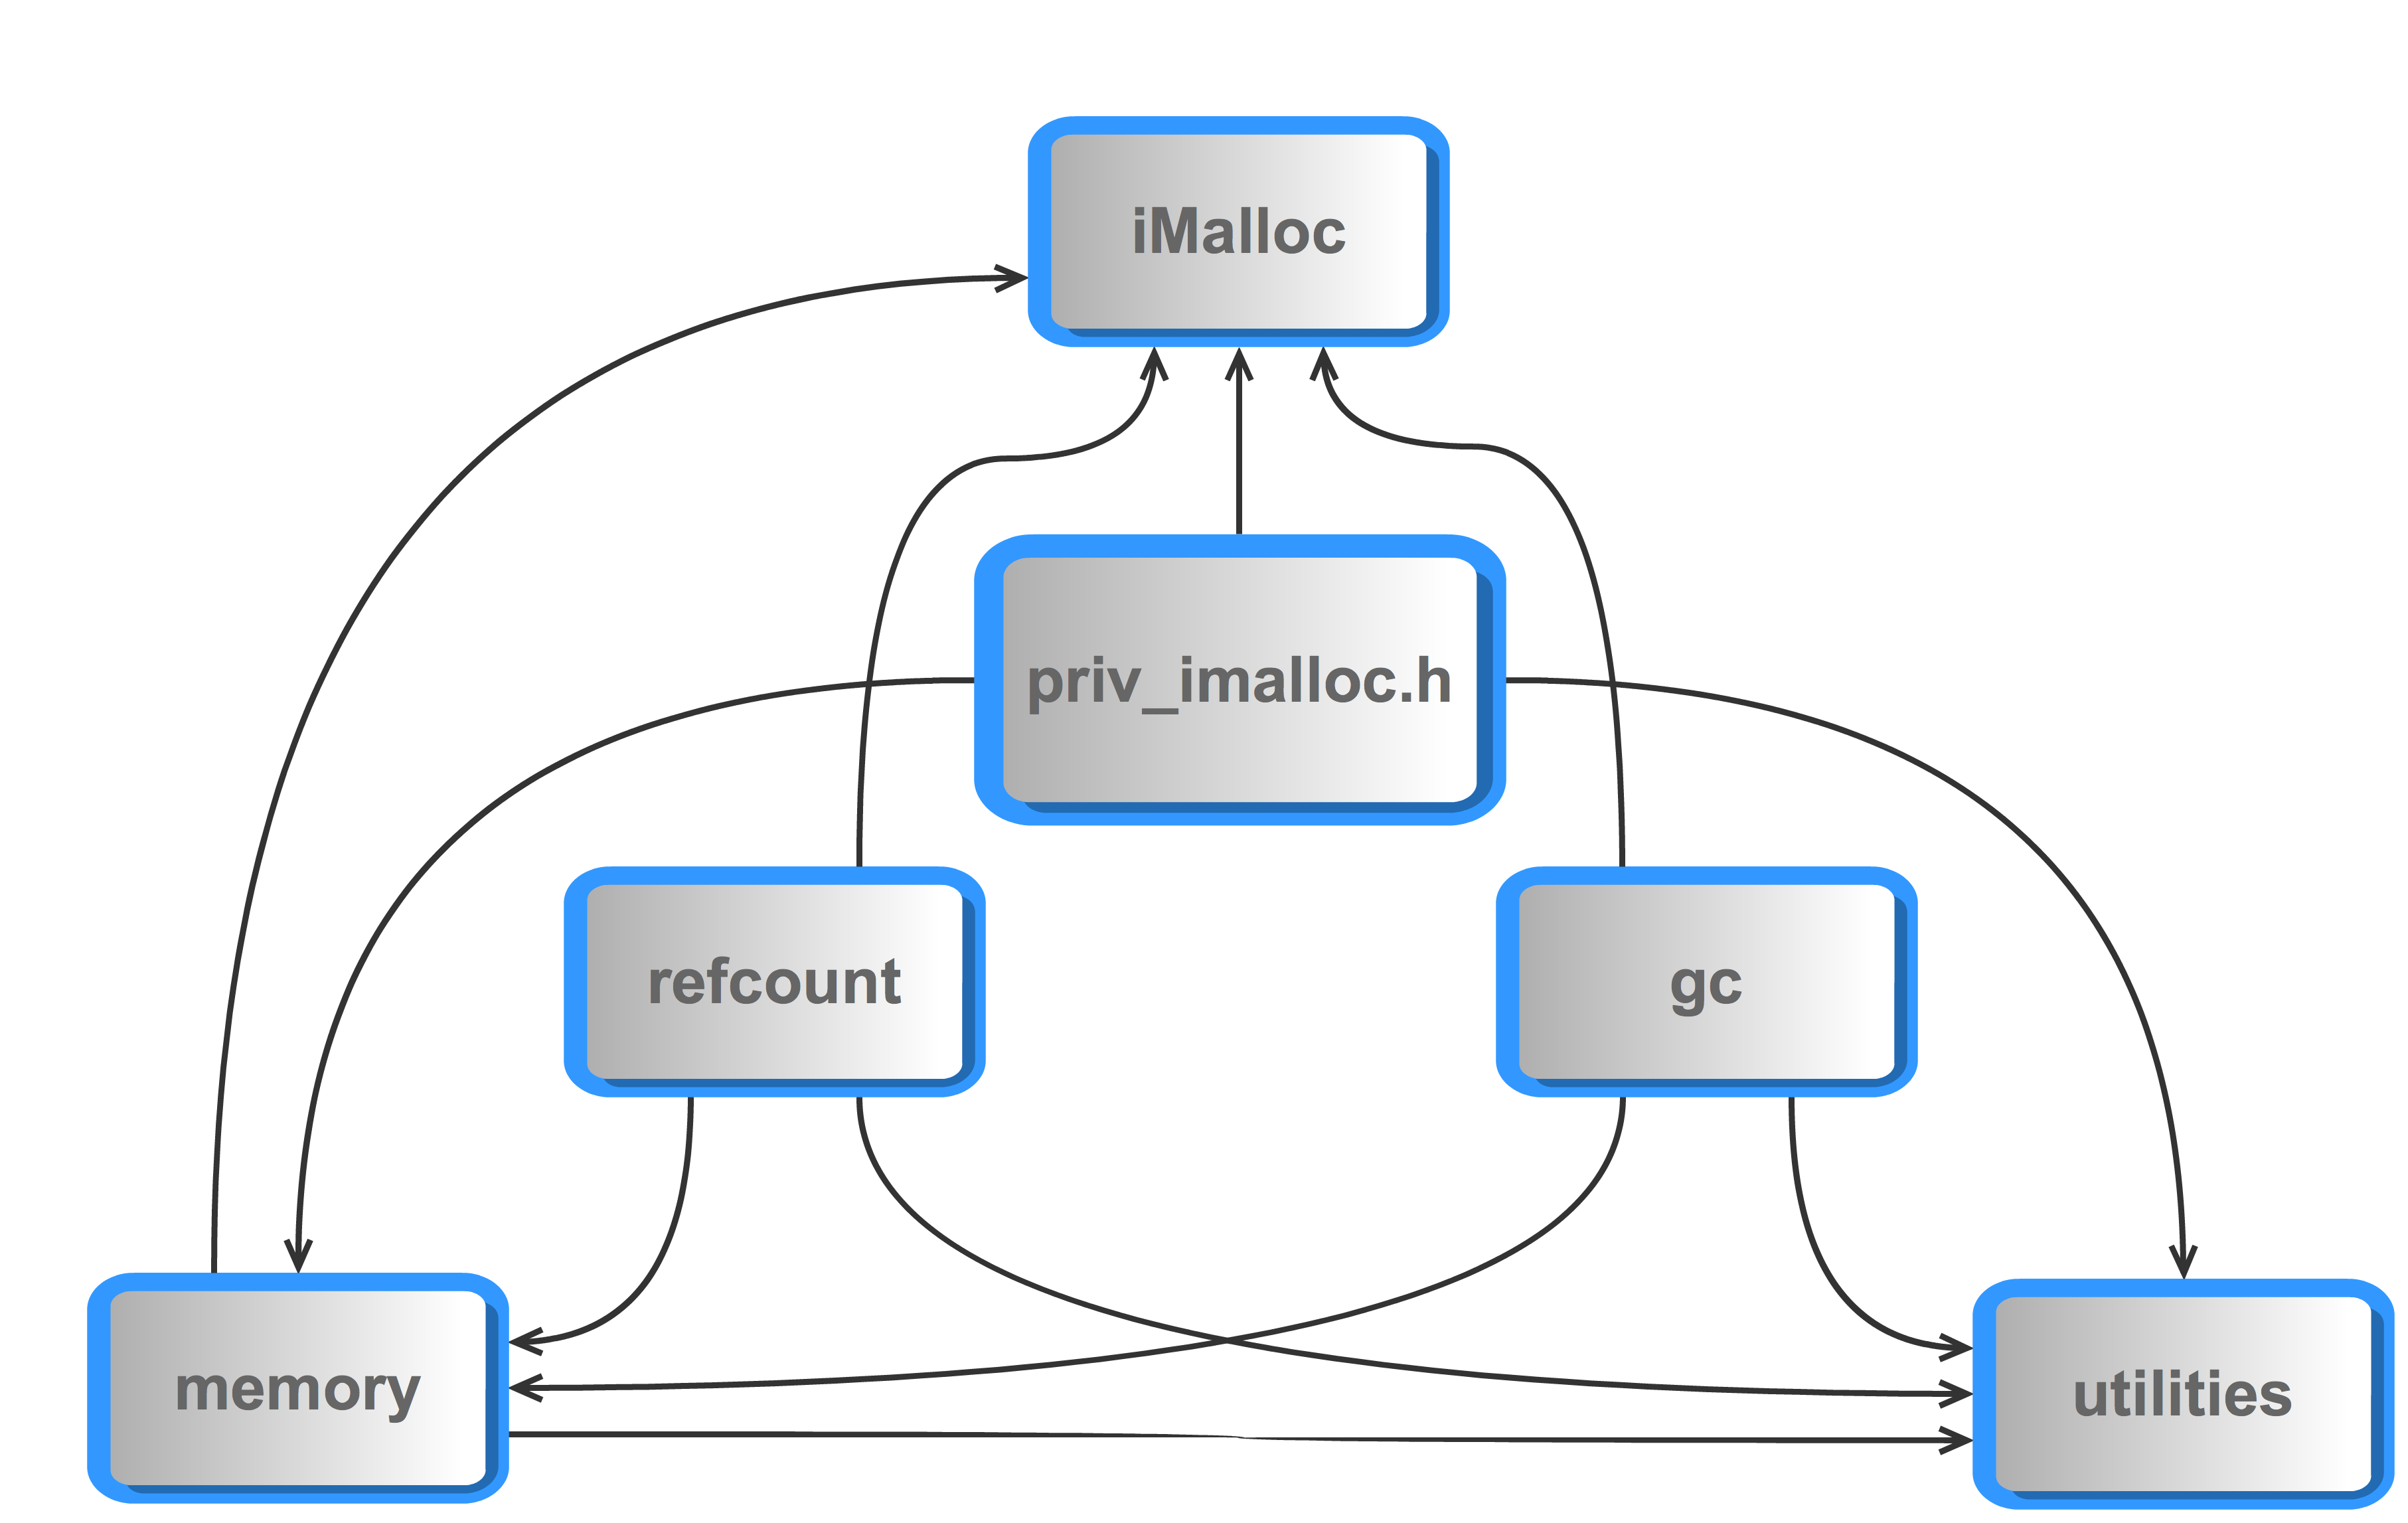
\includegraphics[width=\columnwidth]{images/design_overview.png}
  \caption{Den övergripande designen för programmet.}
  \label{fig:design_overview}
\end{figure}



Här nedan är ett flödesschema på lägre nivå, en mer detaljerad beskrivning av vad hjälpfunktionerna till priv\_imalloc gör och hur de kommunicerar med varandra.

manual, refcount och gc anropar alla varsin typ av alloc. I fallet för gc kan den anropa både typed Alloc eller managed Alloc, beroende på hur input-flaggorna ser ut. typed Alloc gör samma sak som managed Alloc bara att den första gör ett anrop till format för att få ut rätt storlek på formatsträngen.

Samtliga “special Allocs” använder sig av den universala iAlloc.


\begin{figure}[H]
  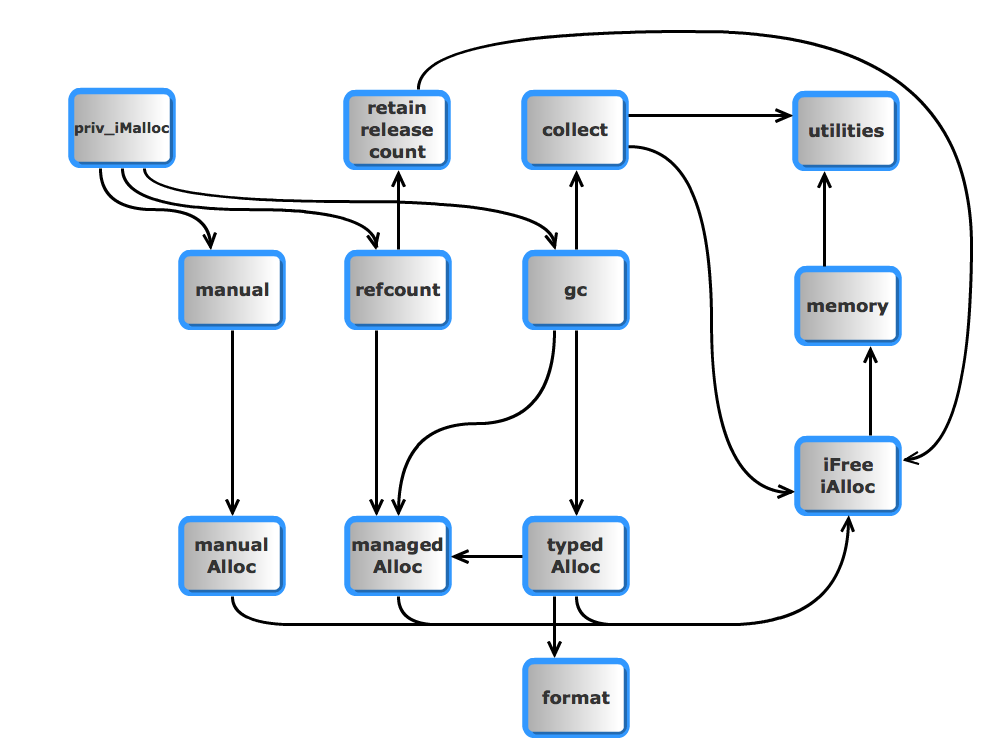
\includegraphics[width=\columnwidth]{images/design_depth.png}
  \caption{En mer djupgående beskrivning av vår design.}
  \label{fig:design_depth}
\end{figure}


\section{Koddokumentation på gränssnittsnivå}
\label{appendix:code}
\documentclass{article}


% This is now the recommended way for checking for PDFLaTeX:
\usepackage{ifpdf}

% Use utf-8 encoding for foreign characters
\usepackage[utf8]{inputenc}

% Swedish grammar
\usepackage[swedish]{babel}

\usepackage[a4paper]{geometry}

% Space between paragraphs instead of indentation.
\usepackage{parskip}

\usepackage{listings}

\usepackage{fancyvrb}
\DefineShortVerb{\|}

\ifpdf
\usepackage[pdftex]{graphicx}
\else
\usepackage{graphicx}
\fi

\ifpdf
\DeclareGraphicsExtensions{.pdf, .jpg, .tif, .png}
\else
\DeclareGraphicsExtensions{.eps, .jpg}
\fi

\usepackage{float}

\pdfpxdimen=1in
\divide\pdfpxdimen by 300

\title{
  Projekt iMalloc \\
  Koddokumentation på gränssnittsnivå
}
\author{
  Niclas Edenvin \\
  Åke Lagercrantz \\
  Andreas Lelli \\
  Daniel Lindgren \\
  Elias Lundeqvist \\
  Jakob Sennerby
}

\date{2012-11-09}



\begin{document}

\maketitle

\newpage

\section{iMalloc}

\subsection*{Synopsis}
\begin{verbatim}
#include imalloc.h
struct style *iMalloc(chunk_size memsiz, unsigned int flags);
\end{verbatim}

\subsection*{Description}

iMalloc returns a pointer to a struct with memsiz reserved memory. 
iMalloc behaves differently depending on which flags has been chosen, 
the flags chose which functions to call.

memsiz is the user defined memory size and the flags changes
the way the memory is behaving and which functions to use.

\subsubsection*{memsiz} The number of bytes you want to reserve which can be entered in several forms.

|1Mb| - Reserves 1 megabyte of memory \\*
|1Kb| - Reserves 1 kilobyte of memory \\*
|10| - Reserves 10 bytes of memory \\*
|sizeof(int)*10| - Reserves enough memory to store 10 integers
\subsubsection*{flags}
Flags are entered separated by a plus sign. Eg. ASCENDING\_SIZE+GCD
The possible flags to choose from is listed below:


{\bf First} Choose how the freelist should be sorted

|ASCENDING_SIZE| - Sort the list with small objects first, large objects in the end \\*
|DESCENDING_SIZE| - Large objects first, small objects in the end \\*
|ADDRESS| - Sort the list depending on their adress, low adresses first, higher towards the end


{\bf Second} Choose which kind of memory manager to use (Note: only REFCOUNT and GCD can be combined)

|MANUAL| - Memory allocation using alloc and free \\*
|REFCOUNT| - Managed memory allocation using reference counter \\*
|GCD| - Managed memory allocation using the mark and sweep algorithm for garbage collection

Any other combinations will produce unspecified results and we cannot guaranty functionality
in those cases.

Usage examples:
Memory with a size of 2Mb, a freelist sorted after descending size and with garbage collection;
|iMalloc(2Mb, ASCENDING_SIZE+GCD)|

Memory with a size of |sizeOf(int)*10|, a freelist sorted after adress and refcount combined with GCD;
|iMalloc(sizeOf(int)*10, ADRESS+GCD+REFCOUNT)|


\section{Structs}
\subsection*{Synopsis}
\begin{verbatim}
typedef struct {
  TypedAllocator alloc;
  Global         collect;
} GC;
\end{verbatim}
\subsection*{Description}
alloc is a pointer to a function used to allocate memory within the adress space created by the iMalloc function.
collect is a pointer to a function used to start a garbage-collecting process according to the mark- and sweep algorithm.

\subsection*{Synopsis}
\begin{verbatim}
typedef struct {
  Local       retain;
  Manipulator release;
  Local       count;
} Refcount;
\end{verbatim}
\subsection*{Description}
This struct is used if a memory object is using refcount.
retain is used to increment the refcount
release is used to decrease the refcount
count returns the current refcount value

\subsection*{Synopsis}
\begin{verbatim}
typedef struct {
  RawAllocator alloc;
  Global       avail;
  Manipulator  free;
} manual, *Manual; 
\end{verbatim}
\subsection*{Description}
This struct is used if using manual memory manager.
alloc is a pointer to a function used to allocate memory within the adress space created by the iMalloc function.
avail returns the total size of the free space in the address space.
free frees an object in memory mem and returns the amount of memory freed.

\subsection*{Synopsis}
\begin{verbatim}
typedef struct {
  RawAllocator alloc;
  Refcount     rc;
  GC           gc;
} managed, *Managed;
\end{verbatim}
\subsection*{Description}
This struct is used if using managed memory manager.
alloc is a pointer to a function used to allocate memory within the adress space created by the iMalloc function.
rc is set when using refcount and/or gc is set when using refcount

\subsection*{Synopsis}
\begin{verbatim}
typedef union {
  manual  manual;
  managed managed;
} style;
\end{verbatim}
\subsection*{Description}
The style union is used as the return value from iMalloc(). This is to allow a return value of either a manual or managed memory manager, without using up unnecessary memory.
After calling iMalloc, you should immediately cast the return value to either a Manual or Managed pointer, like this.
\begin{verbatim}
Manual mem = (Manual) iMalloc(1 Mb, MANUAL + ASCENDING_SIZE);
\end{verbatim}

\section{Typedefs} 
\begin{verbatim}
typedef struct style *Memory;
typedef void *(*RawAllocator)(Memory mem, chunk_size size);
typedef void *(*TypedAllocator)(Memory mem, char* typeDesc);
typedef unsigned int(*Manipulator)(Memory mem, void *ptr);
typedef unsigned int(*Global)(Memory mem);
typedef unsigned int(*Local)(void *ptr);
\end{verbatim}

\end{document}
\section{Gränssnitten mellan modulerna}
\label{appendix:interface}
\documentclass{article}


% This is now the recommended way for checking for PDFLaTeX:
\usepackage{ifpdf}

% Use utf-8 encoding for foreign characters
\usepackage[utf8]{inputenc}

% Swedish grammar
\usepackage[swedish]{babel}

\usepackage[a4paper]{geometry}

% Space between paragraphs instead of indentation.
\usepackage{parskip}

\usepackage{listings}

\usepackage{fancyvrb}
\DefineShortVerb{\|}

\ifpdf
\usepackage[pdftex]{graphicx}
\else
\usepackage{graphicx}
\fi

\ifpdf
\DeclareGraphicsExtensions{.pdf, .jpg, .tif, .png}
\else
\DeclareGraphicsExtensions{.eps, .jpg}
\fi

\usepackage{float}

\pdfpxdimen=1in
\divide\pdfpxdimen by 300

\title{
  Projekt iMalloc \\
  Gränssnitten mellan modulerna
}
\author{
  Niclas Edenvin \\
  Åke Lagercrantz \\
  Andreas Lelli \\
  Daniel Lindgren \\
  Elias Lundeqvist \\
  Jakob Sennerby
}

\date{2012-11-09}



\begin{document}

\maketitle

\newpage

\section{Strukter som används i våra privata funktioner}
\begin{description} \parskip0pt
  \item[Lists] - Innehåller två pekare till chunks
    \begin{description} \parskip0pt
      \item[alloclist] - En lista av chunks som svarar mot objekt allokerade på heapen
      \item[freelist] - En lista med chunks som svarar mot det lediga utrymmet på heapen
    \end{description}

  \item[Chunk] - Innehåller pekarna start och next, storleken chunk_size samt mark-biten
    \begin{description} \parskip0pt
      \item[start] - Pekar till starten på objektet (som svarar mot chunken) som allokerats på heapen eller det fria utrymmet på heapen.
      \item[chunk_size] - Storleken på chunken
      \item[next] - Pekare till nästa chunk i listan.
      \item[mark-bit] - TRUE eller FALSE, beroende på om det finns ett program som använder chunken.
    \end{description}

  \item[priv_mem] - Innehåller addressrymden as, listorna lists samt funktionspekare
    \begin{description} \parskip0pt
      \item[AddressSpace] - En strukt som hör till rootset. Den håller koll på starten och slutet på det utrymme som allokerats med hjälp av imalloc.
      \item[lists]- Innehåller en pekare till strukten lists som i sin tur innehåller pekare till alloclistan och freelistan.
      \item[Funktionspekare] - 
    \end{description}

  \item[AddressSpace] - Innehåller två stycken char-pekare
    \begin{description} \parskip0pt
      \item[start] - En pekare till starten på det allokerade minnet.
      \item[end] - En pekare till slutet på det allokerade minnet.
    \end{description}

\end{description}

\section{imalloc}


\end{document}
\section{Reflektion}
\label{appendix:reflection}
\documentclass{article}


% This is now the recommended way for checking for PDFLaTeX:
\usepackage{ifpdf}

% Use utf-8 encoding for foreign characters
\usepackage[utf8]{inputenc}

% Swedish grammar
\usepackage[swedish]{babel}

\usepackage[a4paper]{geometry}

% Space between paragraphs instead of indentation.
\usepackage{parskip}

\ifpdf
\usepackage[pdftex]{graphicx}
\else
\usepackage{graphicx}
\fi

\ifpdf
\DeclareGraphicsExtensions{.pdf, .jpg, .tif, .png}
\else
\DeclareGraphicsExtensions{.eps, .jpg}
\fi

\usepackage{float}

\pdfpxdimen=1in
\divide\pdfpxdimen by 300

\title{
  Projekt iMalloc \\
  Reflektion
}
\author{
  Niclas Edenvin \\
  Åke Lagercrantz \\
  Andreas Lelli \\
  Daniel Lindgren \\
  Elias Lundeqvist \\
  Jakob Sennerby
}

\date{2012-11-08}



\begin{document}

\maketitle

\newpage

% *********************
% Infoga bild

% se Figur \ref{fig:stable}.

%\begin{figure}[H]
%  \includegraphics[width=165mm]{stabil.png}
%  \caption{Den slutliga versionen av kretsen i Logisim.}
%  \label{fig:stable}
%\end{figure}


% *************************************************************************
% *************************************************************************
% *************************************************************************
% *************************************************************************

Projektet kändes till en början väldigt rörigt. Efter att ha arbetat med att strukturera upp projektet blev det desto tydligare. Det var mycket i projektet som kändes främmande, vilket gjorde allt aningen jobbigt, men av samma anledning var det något vi visste skulle vara väldigt lärorikt. 

Det var svårt att få en känsla av hur uppgiften skulle kunna komma till användning i praktiken, och verkade därför inte så rolig, om man jämför med ett projekt i en tidigare programmeringskurs i ML så gjorde vi ett schackspel, något som efter projektets gång tydligt visade hur bra man hade lyckats och hur det var tänkt att användas. Specifikationen för projektet kändes bra skriven till en början men ju längre projektet fortlöpte desto fler brister fann vi i den. Det saknades en hel del information som vi var tvungna att fråga om i efterhand.

Vi valde att använda oss av Git för vårt arbete. Det blev just Git för att både Niclas och Åke använt det tidigare och var mycket nöjda. Det gjorde också att det gick väldigt snabbt att komma igång med det i hela gruppen. Git gjorde det väldigt smidigt att arbeta på olika delar av programmet samtidigt. Genom att använda olika “brancher” för olika delar kan båda personer i respektive par “commita” i sin branch utan att det påverkar master-branchen, som vi hela tiden har hålt fri från inkomplett kod.

Trello är en webbbaserad tjänst där vi kunnat rita upp en “anslagstavla”. På anslagstavlan skrev vi in vad som behövdes göras, vad som är gjorts och vilka som skulle göra vad:

\begin{figure}[H]
  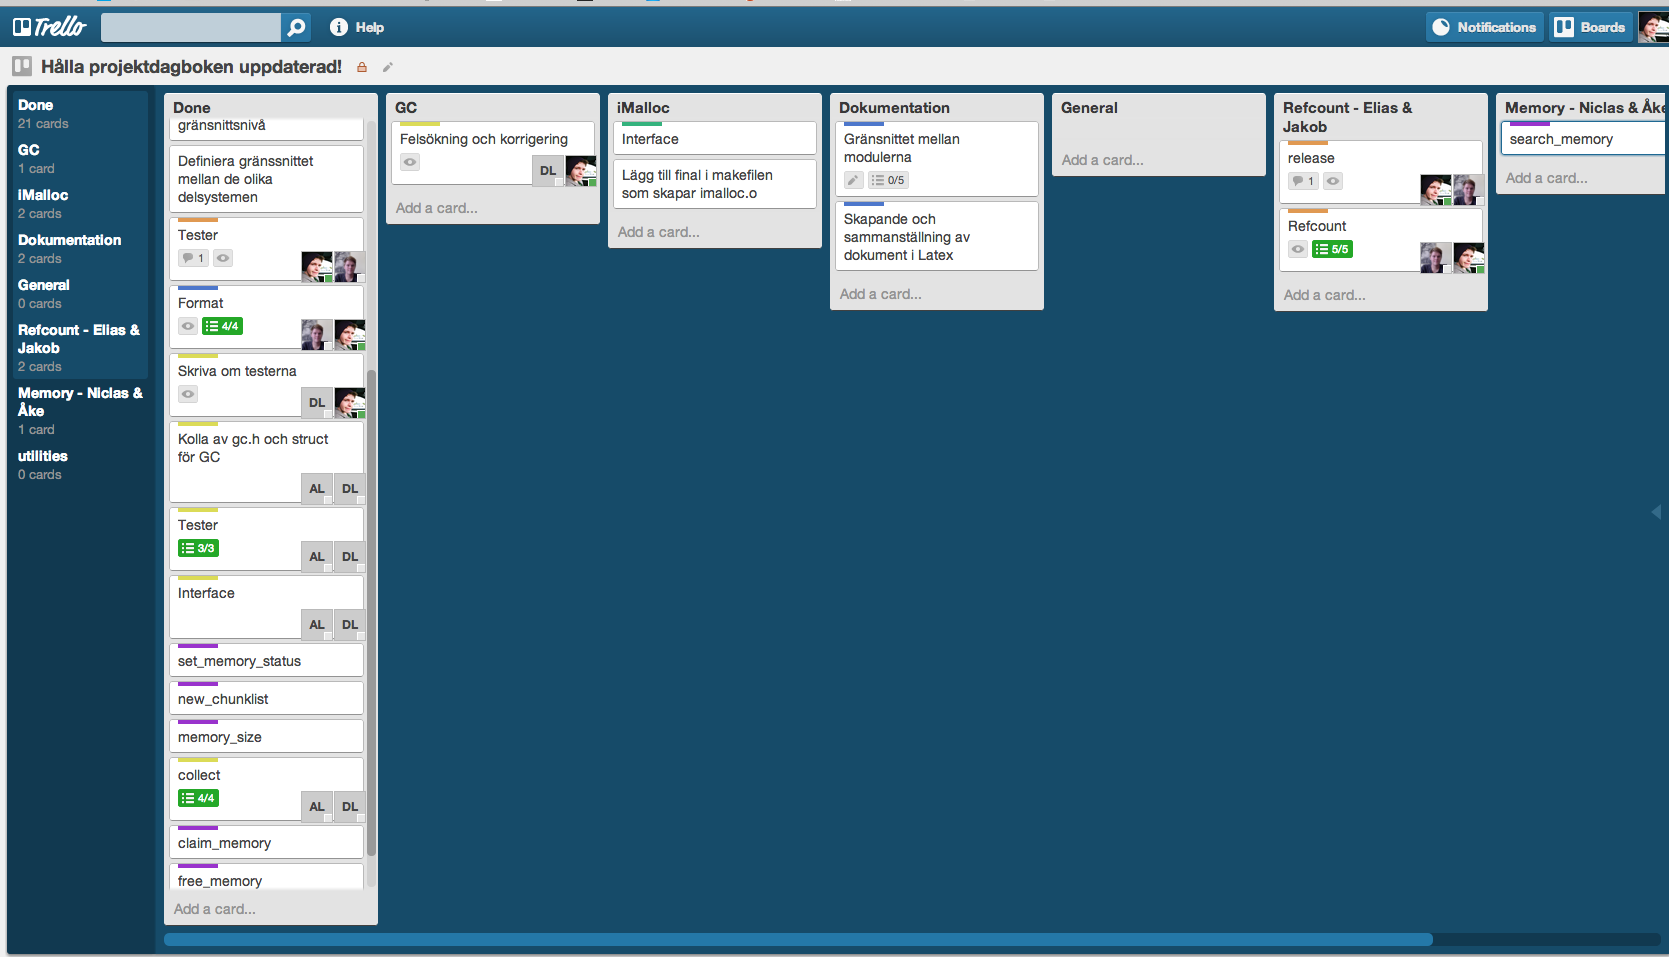
\includegraphics[width=\columnwidth]{../bilder/trello.png}
  \caption{En skärmdump över vår trellotavla den sista veckan.}
  \label{fig:trello}
\end{figure}

Trello har varit en väldigt bra tjänst för att få översikt över projektet. Ville man jobba hemma så var det bara att se på anslagstavlan hur vi låg till och sedan arbeta vidare. Vi delade upp våra mål i små delmål som vi “bockade” av eftersom, vilket gav oss drivkraft att arbeta hårdare och fort gå vidare till nästa delmål.


Varje vardag har vi haft grupprum bokat mellan kl 8 och 17. Det har varit bra att ha som inställning och utgångspunkt - att vi ska jobba åtta timmar varje dag, ibland har någon behövt komma senare eller gå tidigare, därför har vi haft flextider. Det sista varje medlem gjorde innan de gick hem för dagen var att tidsrapportera och skriva dagbok, detta för att ständigt ha koll på vad som har blivit gjort.

I grupprummet har vi alltid haft tillgång till en whiteboard tavla, detta har vart fördelaktigt när någon har stött på problem då alla gruppmedlemmar har kunnat vara med och bolla idéer.Generellt sett har vi försökt arbeta i par så mycket det går men efter att de större delarna av programmet var klara var det svårare att dela upp arbetsuppgifterna på ett jämnt sätt, vi roterade paren trots detta men var inte rädda för att hjälpa varandra och vara lite mer flexibla i vilka uppgifter varje individ arbetade med. 

Något vi har lagt mycket vikt på under hela projektet men framför allt mot slutet var att alla skulle vara informerade av vad alla jobbade med för att således få sig en bra överblick av hur projektet fortskred. 

Diagrammen stämmer inte helt och hållet på grund av vårt sätt att jobba. Eftersom vi satt tillsammans så var ofta alla med och diskuterade fram lösningar på de problem som dök upp. De små avvikelserna tog vi inte hänsyn till när vi valde kategori att tidsrapportera till.

Tidsrapporteringen stämmer inte fullt ut då vi inte har räknat med den tid vi indirekt har arbetat med de olika programdelarna, tex. när man har hjälpt varandra, istället har vi bara i slutet av dagen rapporterat det man har arbetat med i stora drag.


\end{document}




\end{document}

